\chapter{System Design and Dataset}
\label{chap:system}
\begingroup
\justifying
\setlength{\parindent}{2em}
\setlength{\parskip}{0.55\baselineskip}

\section{Design requirements}

Evaluating mobile manipulation in a retail store seems deceptive at first glance. Position a mobile robot before a grocery display, prompt it to retrieve a box of cereal, and watch where execution falters. In simulation, that initial impression of simplicity evaporates almost immediately. Shelves pack hundreds of distinct meshes into narrow clearances. Refrigerator doors impose non-linear kinematic hinges. Mobile bases drift over long trajectories. Dense visual clutter easily overwhelms naive spatial representations. When an episode collapses, the failure must be diagnostic rather than opaque: we need to know whether the policy failed to ground the text prompt, misjudged the pre-grasp offset, lost friction mid-transport, or collided with an adjacent box.

Reproducing and verifying the RoboBenchMart benchmark~\cite{soshin2025robobenchmart} within ManiSkill3~\cite{taomaniskill3} required analyzing the entire system backwards from the demands of physical evaluation. A credible testbed must reconcile several competing engineering imperatives. Scenes must exhibit structural diversity without collapsing into geometric chaos: randomized floor plans must yield navigable aisles and physically plausible fixture alignments rather than arbitrary obstacle mazes. Generation must be strictly deterministic and inspectable, substituting stored, hash-indexed configuration files for unlogged chains of pseudorandom numbers. At the task boundary, success predicates cannot rely on simple bounding-box displacements; they must enforce rigorous collateral checks and stability conditions. Upstream demonstration synthesis must scale without demanding hundreds of hours of manual teleoperation. Finally, the policy interface must present a standardized observation--action contract capable of ingesting models as structurally divergent as diffusion transformers and autoregressive vision--language backbones.

These requirements crystallize into the five-layer decoupled architecture of the reproduced benchmark:
\begin{enumerate}[label=(\roman*),leftmargin=2.5em,itemsep=0.2em]
  \item \textbf{Scene Synthesis Layer}: Translates procedural store boundaries into collision-free fixture layouts and populated shelf inventories.
  \item \textbf{Simulation Environment Layer}: Instantiates the synthesized store within ManiSkill3, binds the Fetch mobile manipulator, configures lighting, and computes physical contacts.
  \item \textbf{Demonstration Generation Layer}: Leverages privileged simulator state, analytical kinematics, and motion planning to generate collision-free supervision trajectories.
  \item \textbf{Policy Evaluation Interface}: Exposes a multi-view visual and language-conditioned client, abstracting simulator specifics behind standardized sensor buffers.
  \item \textbf{Diagnostic Analysis Layer}: Evaluates terminal task predicates, monitors non-target disturbances, logs trajectory failures, and categorizes failure modalities.
\end{enumerate}

Decoupling these subsystems is an essential architectural decision. By isolating scene synthesis from policy rollouts, individual floor plans can be rendered, audited, and visually inspected long before any model consumes compute. Separating task predicates from learned controllers guarantees that ground-truth metrics remain strictly unpolluted by policy idiosyncrasies. Most critically, an identical library of frozen procedural seeds can be presented across every baseline architecture, ensuring that downstream performance variations reflect policy behavior rather than stochastic fluctuations in the environment.

\section{Store-plan generation}

A physical supermarket is not an unstructured scattering of furniture; it is an optimized topological network of parallel aisles, perimeter boundaries, and focal displays. To capture this spatial grammar procedurally, the generator models a store as a bounded two-dimensional polygonal floor plan $\Omega \subset \mathbb{R}^2$ populated by primary fixtures and structural obstacles. 

The generation pipeline executes in two successive passes. In the first pass, structural obstacles, structural columns, and large boundary fixtures are positioned via rejection sampling. Candidate footprints that intersect existing geometry or breach minimal clearance envelopes are discarded. This initial placement establishes the primary geometric contours that govern subsequent retail circulation.

The second pass synthesizes internal shelving runs by querying a continuous orientation field derived from boundary geometry. Let the store boundary and obstacle perimeters be represented by closed polygonal curves $\{\mathbf{p}_i\}_{i=1}^{P}$. Define directed edge vectors $\mathbf{u}_i = \mathbf{p}_{i+1} - \mathbf{p}_i$, with cyclic closure $\mathbf{p}_{P+1} = \mathbf{p}_1$. To prevent long wall segments from dominating local calculations, edges exceeding a threshold length $D$ are recursively subdivided. Each boundary segment, characterized by orientation $\theta_i = \operatorname{atan2}(u_{i,y}, u_{i,x})$ and length $\ell_i = \lVert\mathbf{u}_i\rVert_2$, induces an elementary symmetric traceless tensor:
\begin{equation}
  \mathbf{T}_i = \ell_i
  \begin{bmatrix}
  \cos(2\theta_i) & \sin(2\theta_i)\\
  \sin(2\theta_i) & -\cos(2\theta_i)
  \end{bmatrix}.
  \label{eq:basis-tensor}
\end{equation}
The doubled angle maps opposite directions to identical tensor representations, encoding an undirected axial orientation invariant to whether an edge is traversed clockwise or counterclockwise. For any floor query coordinate $\mathbf{x} \in \Omega$, the aggregated tensor field is computed via exponential distance decay:
\begin{equation}
  \mathbf{T}(\mathbf{x}) = \sum_i
  \exp\!\left(-d\,\lVert\mathbf{x}-\mathbf{p}_i\rVert_2\right)\mathbf{T}_i,
  \label{eq:tensor-field}
\end{equation}
where the decay parameter $d > 0$ determines the spatial decay rate of contour influence. The eigenvectors of $\mathbf{T}(\mathbf{x})$ define the locally dominant principal axes.

Because symmetry and tracelessness are preserved under linear combination, the accumulated tensor retains the canonical form:
\begin{equation}
  \mathbf{T}(\mathbf{x}) =
  \begin{bmatrix}
  a(\mathbf{x}) & b(\mathbf{x})\\
  b(\mathbf{x}) & -a(\mathbf{x})
  \end{bmatrix}.
\end{equation}
The dominant axial orientation $\theta^{\star}(\mathbf{x})$ is recovered analytically without full eigendecomposition:
\begin{equation}
  \theta^{\star}(\mathbf{x}) = \frac{1}{2}\operatorname{atan2}\!\left(b(\mathbf{x}),\,a(\mathbf{x})\right).
  \label{eq:tensor-orientation}
\end{equation}
This closed-form formulation reveals the underlying computational complexity. Evaluating Equation~\ref{eq:tensor-field} across $G$ floor query cells against $J$ discretized boundary samples scales as $\mathcal{O}(GJ)$ in time, with $\mathcal{O}(G)$ memory overhead. In a naive implementation, this cost scales directly with room perimeter and obstacle density. In the benchmark implementation, candidate queries are evaluated lazily along discrete sweep trajectories, avoiding exhaustive grid precomputation.

A minimal numerical example illuminates the tensor aggregation. Consider a horizontal boundary segment of length 2 passing directly through the query point ($\theta_H = 0$, $\ell_H = 2$, distance $0$), and an orthogonal vertical segment of length 1 located at a perpendicular distance of 1 unit ($\theta_V = \pi/2$, $\ell_V = 1$). Setting the decay parameter $d = 1$, their respective tensor contributions are:
\begin{equation}
  \mathbf{T}_{H} = 2
  \begin{bmatrix}1 & 0\\ 0 & -1\end{bmatrix},
  \qquad
  \mathbf{T}_{V} = e^{-1}
  \begin{bmatrix}-1 & 0\\ 0 & 1\end{bmatrix}.
\end{equation}
Summing these contributions yields:
\begin{equation}
  \mathbf{T}_{H} + \mathbf{T}_{V}
  = \begin{bmatrix}2 - e^{-1} & 0\\ 0 & -(2 - e^{-1})\end{bmatrix}
  \approx \begin{bmatrix}1.632 & 0\\ 0 & -1.632\end{bmatrix}.
\end{equation}
Applying Equation~\ref{eq:tensor-orientation} gives $b(\mathbf{x}) = 0$ and $a(\mathbf{x}) > 0$, producing $\theta^{\star} = 0^{\circ}$. The horizontal orientation dominates because the proximal, longer boundary outweighs the orthogonal segment.

In practice, the tensor field acts as a directional filter rather than a continuous protractor. Candidate fixtures are evaluated along orthogonal horizontal and vertical sweep vectors across the floor. Rather than rotating a shelf continuously to match $\theta^{\star}(\mathbf{x})$, the local orientation is tested against the Cartesian axes. If the principal direction falls within approximately $37^{\circ}$ of a coordinate axis, the candidate fixture is snapped to that axis. Consequently, every fixture in the synthesized store is strictly axis-aligned. The tensor field determines where an axis-aligned unit may reside, not its continuous heading. Candidate acceptance further demands an intersection-free footprint, compliance with a 2.0-meter passage envelope, and passage through an independent Bernoulli trial with a skip probability of $0.1$ to break rigid uniformity.

Moreover, the decay coefficient is configured to $d = 12$. At a radial distance of $r = 0.5$~meters, the exponential weight $\exp(-12 \times 0.5) \approx 0.0025$, collapsing the effective influence radius to approximately thirty centimeters. As a result, the orientation gate is almost entirely dictated by the single nearest boundary contour rather than a blended consensus of distant walls. The resulting floor plans achieve regular, well-separated aisle rows following perimeter geometries, but the underlying mechanism is an axis-snapped spatial gate rather than a continuous fluid field.

\begin{figure}[H]
    \centering
    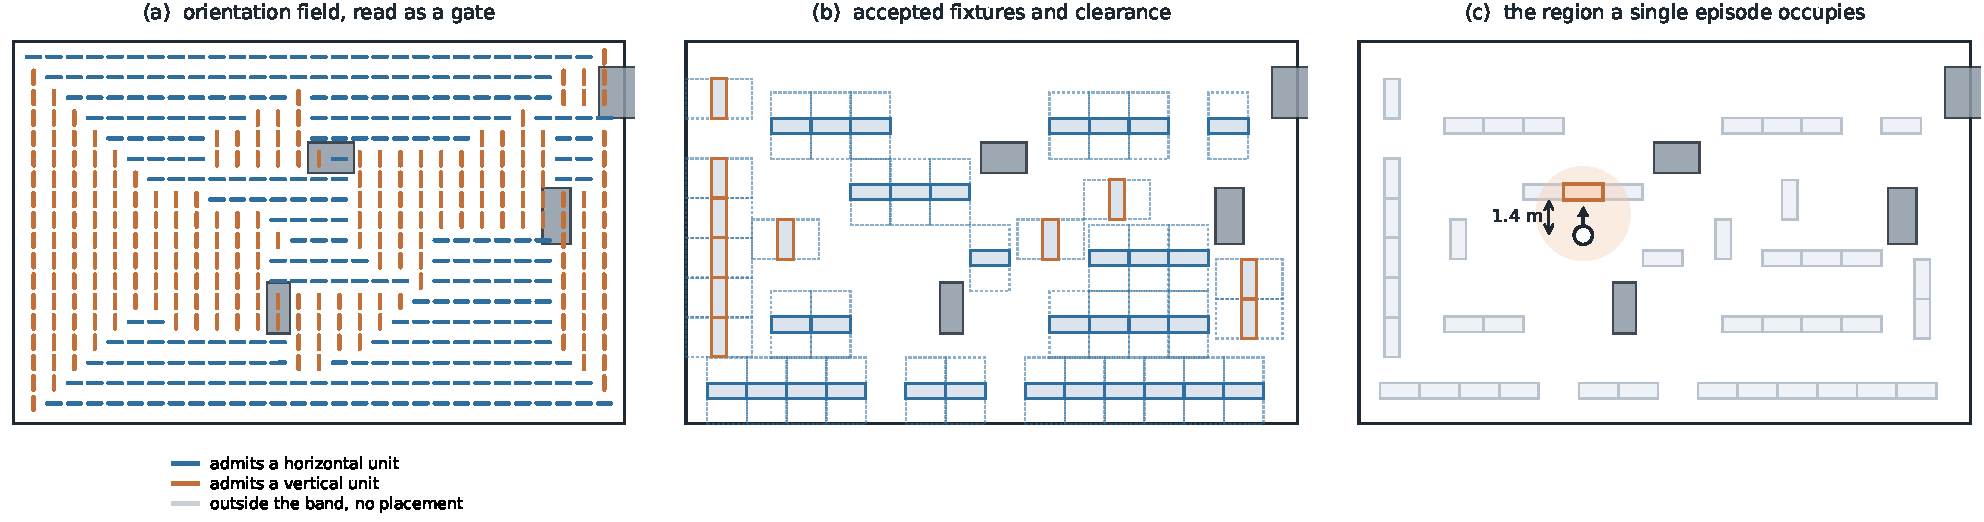
\includegraphics[width=\textwidth]{assets/figures/retail-vla-benchmark/layout_pipeline.pdf}
    \caption{Store generation pipeline for a $24\times15$~m retail space at $d=12$. (a) The discrete orientation field sampled across floor coordinates, displayed as unsigned axial ticks colored by acceptance gating. (b) Synthesized layout after collision, clearance, and passage rejection; units concatenate longitudinally to form multi-shelf runs. (c) Local episode footprint showing the active shelving unit, the robot's initial base placement at 1.4~m, and the operational workspace traversed during interaction. The simulation generates a multi-aisle supermarket, but policy execution remains confined to a local floor patch.}
    \label{fig:store-generation}
\end{figure}

\ref{fig:store-generation} illustrates the full synthesis progression. Panel (a) shows the orientation field sampled across a regular floor grid. Because the room boundaries are rectilinear, the field aligns with the coordinate axes across the vast majority of the interior. Rejection occurs primarily in regions where competing obstacle geometries induce diagonal vectors that fail the axial acceptance threshold. Panel (b) depicts the surviving store layout, demonstrating coherent multi-unit runs separated by generous aisles. Panel (c) highlights an important physical reality: while the generator synthesizes a comprehensive 360-square-meter supermarket, any single manipulation episode is restricted to a compact interaction envelope directly adjacent to an assigned fixture.

Standardized store environments measure $24 \times 15$~meters. Aisles maintain a minimum passage clearance of $2.0$~meters; free-standing shelving units maintain an occupancy buffer of $1.0$~meter, while wall-adjacent fixtures require $0.4$~meters. Boundary polygons are subdivided at $1.0$~meter intervals, and fixture perimeters at $0.5$~meters. If the procedural placement fails to satisfy valid scene constraints after twenty attempts, the seed is rejected.

Generated store definitions are serialized into compact JSON structures indexed by SHA-1 configuration hashes, enabling asynchronous batch production across multiple processor cores. The configuration schema specifies two distinct pseudorandom seed streams: one for structural floor layout and one for stock arrangement. In the evaluated benchmark configuration, both streams are initialized by adding the scene index to an identical base integer, locking layout and stock variation to the same underlying random sequence.

\section{Products, fixtures and visual variation}

The asset library comprises three commercial shelving units, two refrigerated merchandisers, and 371 retail product meshes spanning 21 retail categories, complemented by 23 legacy assets from preliminary design revisions. Surface materials are sampled from independent texture pools containing 26 floor, 17 wall, and 15 ceiling finishes. As shown in \ref{fig:asset-library}(a), asset distribution across categories is highly non-uniform: hygiene and spirits exceed forty distinct items each, whereas frozen commodities contain only two.

\begin{figure}[H]
    \centering
    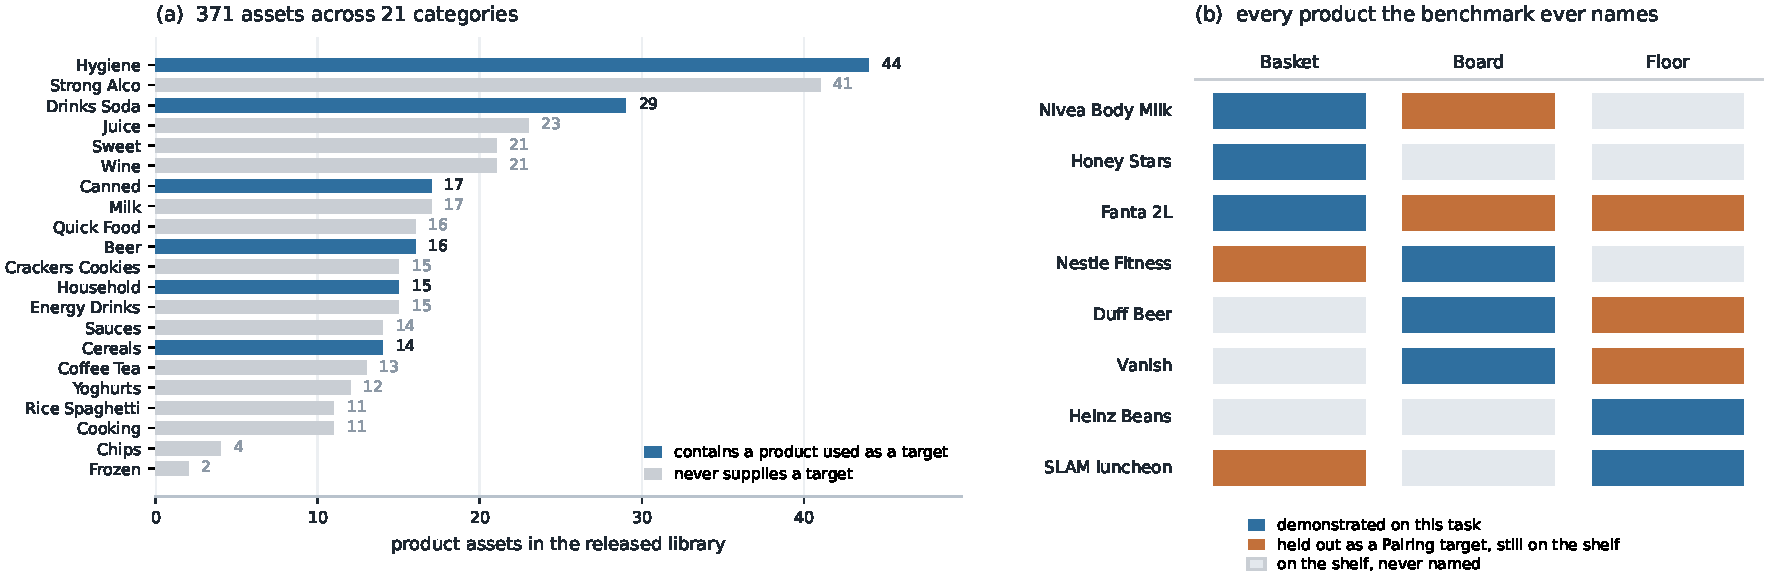
\includegraphics[width=\textwidth]{assets/figures/retail-vla-benchmark/asset_library.pdf}
    \caption{Asset catalogue distribution and evaluation coverage. (a) Total product assets per category across the 371-item catalogue; highlighted bars denote categories containing at least one task target. (b) The eight target products utilized in the evaluation benchmark and their roles across pick-and-place tasks. Crucially, products designated as unseen targets in the Pairing condition remain present as background clutter on training shelves throughout model adaptation.}
    \label{fig:asset-library}
\end{figure}

Panel (b) of \ref{fig:asset-library} reveals a critical boundary condition. Across the entire 371-item library, exactly eight products are ever referenced in task prompts. These eight items originate from six retail categories, and each serves as an interaction target in at most two distinct pick-and-place tasks. While the broader visual library is extensive, the empirical manipulation corridor is narrow. Claims regarding semantic grounding and zero-shot open-vocabulary generalization must be calibrated against this eight-object interaction set rather than the catalogue total.

Furthermore, \ref{fig:asset-library}(b) exposes an essential detail of the compositional evaluation split. A product withheld from task-specific training demonstrations is not absent from the visual world. It sits on the same shelves, rendered under identical lighting and camera perspectives, alongside active items during adaptation. The robot is repeatedly exposed to the visual geometry of these items; what is withheld is the pairing between the item's textual identity and the physical manipulation skill.

Integrating diverse third-party meshes into a rigid-body simulator introduces substantial physical friction. Raw assets sourced from heterogeneous 3D repositories exhibit incompatible dimensional units, non-standardized coordinate origins, and erratic bounding centers. Every asset underwent manual scaling against real-world retail packaging dimensions, orientation normalization, and support-surface annotation. Without accurate geometric scaling, gripper grasp envelopes and kinematic reachability checks become physically meaningless.

High-polygon meshes present an even steeper computational barrier. Retail packaging meshes frequently carry tens of thousands of triangles. Populating dozens of shelving units with unoptimized geometry instantly overwhelms GPU memory and collapses simulation throughput. To resolve this bottleneck, the benchmark deploys an automated mesh decimation pipeline incorporating QuadriFlow quadrangulation, Marching Cubes surface extraction, and primitive bounding proxies (boxes, cylinders). Candidate geometries are evaluated by measuring geometric deviation against the source mesh via Chamfer distance versus the remaining triangle budget.

\begin{figure}[H]
    \centering
    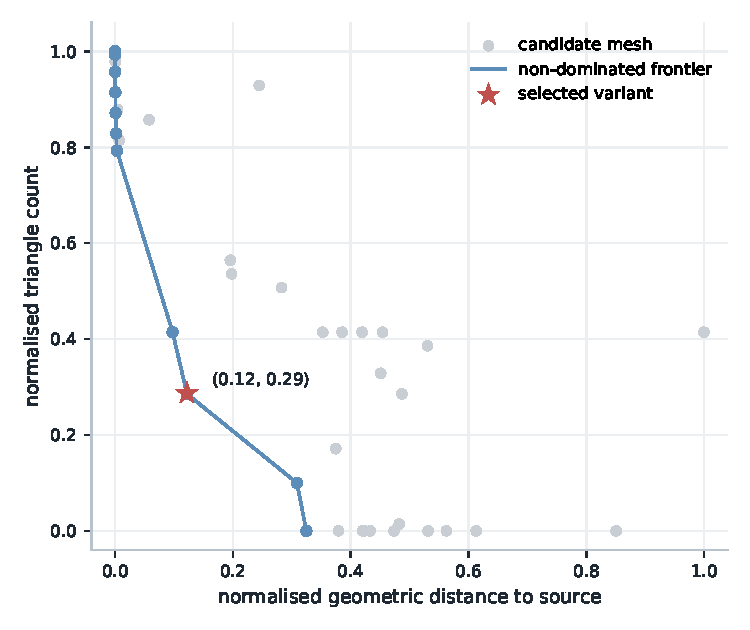
\includegraphics[width=0.62\textwidth]{assets/figures/retail-vla-benchmark/asset_pareto.pdf}
    \caption{Multi-objective mesh simplification Pareto frontier for a representative retail asset, normalized on both axes (lower is preferred). Out of 43 candidate approximations generated via QuadriFlow and decimation filters, eleven form the non-dominated Pareto frontier. A steep knee occurs at $(0.12,\,0.29)$, where triangle count drops by 71\% while preserving 88\% of source geometric fidelity.}
    \label{fig:asset-pareto}
\end{figure}

Selection cannot rely on a naive decimation ratio. As illustrated in \ref{fig:asset-pareto}, geometric error and polygon counts form a non-linear Pareto trade-off. Primitive geometric envelopes minimize polygon counts to negligible levels but obliterate distinctive product silhouettes, rendering visual grounding impossible. Conversely, aggressive remeshing algorithms occasionally increase triangle density without reducing Chamfer error. Across 43 evaluated simplification candidates, eleven reside on the non-dominated Pareto frontier. The optimal candidate was selected at the sharp knee of the curve, retaining 29\% of the original triangle count while incurring only 12\% of the maximum observed Chamfer error. Simplified proxies are deployed across all background fixtures, whereas foreground targets maintain high-fidelity collision envelopes.

Shelf population proceeds across identified horizontal support planes. Stock items are placed on a structured Cartesian grid subject to bounded translational and rotational perturbations ($\pm 1.5$~cm, $\pm 5^{\circ}$). This produces the dense visual arrangement characteristic of commercial grocery displays. While procedural mechanisms for vertical product stacking and Poisson-process stock depletion were formulated in initial design specifications, neither was deployed in the experimental environment. Every training and evaluation scene in this dissertation is fully packed.

\section{Robot and task environments}

Physical manipulation is simulated using the Fetch mobile manipulator in ManiSkill3~\cite{taomaniskill3}. The Fetch platform integrates a differential-drive mobile base for planar navigation, a prismatic torso joint providing vertical reach adjustment, a 7-degree-of-freedom articulated arm, and a two-finger parallel-jaw gripper. ManiSkill3 provides GPU-accelerated rigid-body dynamics, contact mechanics, and batch rendering.

The benchmark defines five canonical atomic tasks:
\begin{enumerate}[label=(\alph*),leftmargin=2.5em,itemsep=0.2em]
  \item \textbf{Pick to basket}: Locate a specified target product on a shelf or merchandiser, extract it from surrounding clutter, and deposit it into the robot's shopping basket.
  \item \textbf{Pick from floor}: Acquire a fallen target item resting on the floor surface and return it to a designated shelf tier.
  \item \textbf{From board to board}: Transfer an item from an upper or lower shelf tier to an alternate level within the same fixture.
  \item \textbf{Open fridge}: Grasp the handle of a refrigerated display door and articulate it past a specified angular opening threshold.
  \item \textbf{Close fridge}: Engage an open refrigerator door and push or swing it back into its fully latched position.
\end{enumerate}
In addition to standard refrigerator units, the codebase incorporates showcase merchandisers featuring four distinct articulated door leaves. These showcase variants share kinematic interaction mechanics with the primary refrigerator doors but specify discrete target handles, expanding the internal task registry beyond the five headline atomic families.

Natural-language prompts specify the target product and fixture description without exposing simulator entity pointers (e.g., \texttt{"pick the green tea box from the second shelf and place it in the basket"}). If duplicate candidate fixtures exist within the store, the policy is expected to navigate to and interact with the closest instance. This structure mirrors human operational instructions while requiring the model to resolve physical grounding autonomously.

Task success predicates enforce strict spatial and kinematic constraints rather than superficial target displacement:
\begin{equation}
  y = \mathbb{I}[o^* \in G]\;\mathbb{I}[\lVert\mathbf{v}_{\text{robot}}\rVert_2 \leq v_{\text{tol}}]\;\prod_{o \in \mathcal{N}(o^*)} \mathbb{I}[\lVert\Delta \mathbf{p}_o\rVert_{\infty} \le \epsilon_p \;\land\; \lVert\Delta \mathbf{q}_o\rVert_{\infty} \le \epsilon_q].
  \label{eq:predicate-success}
\end{equation}
For pick-and-place tasks, the target item $o^*$ must settle within the designated target volume $G$, the robot platform must come to a complete rest ($\lVert\mathbf{v}_{\text{robot}}\rVert_2 \leq 0.2$~m/s), and surrounding collateral objects $\mathcal{N}(o^*)$ must remain undisturbed within translational ($\epsilon_p = 0.1$~m) and rotational ($\epsilon_q = 0.1$) tolerances. In the basket task, $G$ is defined as a $0.4\times 0.4\times 0.4$~m bounding box centered on the onboard basket (expanded to $0.5$~m for large cereal packaging such as Honey Stars), and non-target monitoring is restricted to the active fixture shelf. For board transfer, $G$ specifies a $0.1$-meter horizontal boundary centered $0.397$~meters above the source shelf. For door tasks, success hinges on articulation metrics: showcase doors must reach $1.57 \pm 0.2$~radians (or return to $0 \pm 0.2$~rad for closure), whereas refrigerator covers require reaching $0.624 \pm 0.1$~radians (approximately $35.8^{\circ}$).

Two composite tasks are defined within the upstream RoboBenchMart benchmark to evaluate sequential horizon scaling:
\begin{itemize}[leftmargin=2.5em,itemsep=0.2em]
  \item \textbf{Pick three items}: Sequentially locate, grasp, and deposit three distinct target products into the mobile basket across successive prompt instructions.
  \item \textbf{Pick from fridge}: Execute a three-stage sequential chain: open the refrigerator door, extract the internal target beverage into the basket, and close the door.
\end{itemize}
In the upstream design, an algorithmic oracle monitors the subtask predicate and issues the subsequent natural-language prompt upon verified completion of the preceding stage. While these multi-stage tasks provide a conceptual framework for long-horizon planning, the empirical campaign in this dissertation restricts its scope strictly to atomic primitives, where baseline physical execution can be rigorously isolated and measured.

\section{Training corpus and demonstration provenance}

In the upstream RoboBenchMart framework, supervised training demonstrations were generated algorithmically across twelve canonical task--item--fixture configurations. The upstream collection pipeline captured 248 verified trajectories per triplet, yielding a nominal corpus of 2,976 demonstration episodes and 1,401,169 state--action transitions. In our reproduction environment, the repository preserves the twelve configuration index files and 2,976 episode metadata headers defining these trajectories. However, because local data containers store configuration metadata rather than full continuous state--action sensor arrays, this dissertation does not claim to have generated or trained on a local 1.4-million transition dataset. Instead, this metadata documents the training distribution of the publicly released fine-tuned checkpoints evaluated in Chapter~\ref{chap:results}.

Each transition records three complementary sensory streams:
\begin{itemize}[leftmargin=2.5em,itemsep=0.2em]
  \item \textbf{Language Prompt}: A descriptive task instruction specifying target product and destination fixture.
  \item \textbf{Visual Observations}: Three synchronized RGB camera views, consisting of exterior left-shoulder ($256\times 256\times 3$), exterior right-shoulder ($256\times 256\times 3$), and an eye-in-hand wrist camera ($128\times 128\times 3$). The robot's native head camera was omitted because the Fetch arm frequently blocks its line of sight during close manipulation.
  \item \textbf{Proprioception}: Joint positions and velocities of the 7-DOF arm, parallel gripper, and mobile base.
\end{itemize}

The commanded action is structured as a 13-dimensional continuous vector:
\begin{equation}
  \mathbf{a}_t = \left[\mathbf{q}^{\text{arm}}_t,\ a^{\text{grip}}_t,\ \mathbf{q}^{\text{body}}_t,\ v^{\text{base}}_t,\ \omega^{\text{base}}_t\right] \in \mathbb{R}^{13},
  \label{eq:action-vector}
\end{equation}
comprising seven arm joint target angles $\mathbf{q}^{\text{arm}}_t \in \mathbb{R}^7$, a scalar gripper position command $a^{\text{grip}}_t \in [0, 1]$, three body joint targets $\mathbf{q}^{\text{body}}_t = [q_{\text{torso}}, q_{\text{pan}}, q_{\text{tilt}}] \in \mathbb{R}^3$, and planar base linear and angular velocities $(v^{\text{base}}_t, \omega^{\text{base}}_t)$. Arm and torso joints operate under a proportional-derivative position-target controller, while the mobile base is governed by velocity setpoints.

A critical physical constraint was discovered during our runtime protocol audit. In the experimental evaluation client, the torso-lift and head-pan command dimensions are explicitly overwritten with zero at every simulation step. Because the low-level controller interprets joint setpoints as absolute coordinates rather than incremental displacements, this zero-clamping forces the prismatic torso to remain permanently pinned at its mechanical minimum ($q_{\text{torso}} = 0$). Demonstrations collected by the motion planner were likewise initialized and executed with the torso at zero. Consequently, across every policy, task, and demonstration in this benchmark, the robot operates with an entirely rigid spine. Vertical reach is a frozen constant of the environment, fundamentally constraining the robot's physical reach during floor retrieval and upper-shelf placement.

\section{Design decisions and rejected alternatives}

The technical design of this benchmark reflects deliberate engineering compromises between physical fidelity, computational throughput, and diagnostic clarity.

\textbf{Procedural Stores versus Isolated Shelf Cells.} An alternative approach would decouple manipulation from store environments, evaluating policies exclusively on isolated single-shelf modules. While an isolated shelf reduces rendering overhead and accelerates reset cycles, it destroys the visual and geometric context essential for embodied agents. Whole-store procedural generation forces the policy to operate under realistic visual backgrounds, varying aisle perspectives, and realistic global lighting, while preserving layout coherence for future navigation benchmarks.

\textbf{Serialized Plans versus Online Generation.} Rather than generating floor plans procedurally inside the environment reset loop, layouts are pre-synthesized, verified, and serialized into static JSON configuration files. This separation enables rigorous experimental version control: every model baseline is evaluated against the exact same frozen geometry and initial object poses. Furthermore, failed rollouts can be re-rendered and debugged offline without re-running stochastic generation routines.

\textbf{Continuous Fields versus Discrete Orientation Sweeps.} The theoretical formulation of Equations~\ref{eq:basis-tensor}--\ref{eq:tensor-orientation} allows continuous orientation interpolation. However, continuous shelf angles in a rectilinear retail store produce awkward triangular dead spaces and irregular aisles that fail standard accessibility constraints. The benchmark design therefore restricts the tensor field to act as an acceptance gate along Cartesian sweep vectors, preserving realistic aisle geometries while retaining boundary sensitivity.

\ref{tab:layout-generation-ab} summarizes the analytical trade-offs governing the layout synthesis architecture.

{\renewcommand{\arraystretch}{1.18}
\begin{table}[H]
\centering
\footnotesize
\begin{tabularx}{\textwidth}{
>{\RaggedRight\arraybackslash}p{0.18\textwidth}
>{\RaggedRight\arraybackslash}X
>{\RaggedRight\arraybackslash}X
>{\RaggedRight\arraybackslash}X}
\toprule
Dimension & Handcrafted templates & Unconstrained random placement & Tensor-gated sweep (RoboBenchMart suite) \\
\midrule
Source of order & Static human architectural designs & Independent random coordinates; order emerges only by rare chance & Boundary contours induce continuous axial orientation fields \\
Layout diversity & Restricted to manual permutations and minor parametric offsets & High, but frequently geometrically degenerate & Continuous procedural variation across seeds while preserving aisle corridors \\
Clearance enforcement & Hardcoded during authoring; easily invalidated by scaling & Enforced through brute-force rejection sampling & Rejection sampling guided by directional clearance envelopes \\
Boundary adaptation & Requires bespoke repair scripts for non-rectangular rooms & Geometrically flexible, but generates irregular, disjoint pockets & Automatically aligns runs with non-standard perimeter geometry \\
Computational profile & Negligible runtime; substantial human authoring burden & Inexpensive proposals; rejection rate surges under high spatial packing & $\mathcal{O}(J)$ field evaluations per candidate; easily parallelized across cores \\
Characteristic flaws & Rigid visual repetition; poor coverage of novel layouts & Chaotic fixture angles; unnavigable dead ends; floating geometry & Sensitive to decay parameter $d$, grid stride, and skip probability \\
Unaddressed constraints & Operational logistics, fire codes, and dynamic restock routes & Retail semantics, product adjacency, and physical accessibility & Customer traffic flow, inventory clustering, and operational zoning \\
\bottomrule
\end{tabularx}
\caption{Analytical design comparison of store-layout synthesis paradigms.}
\label{tab:layout-generation-ab}
\end{table}}

\textbf{Sensor Configuration.} The Fetch robot's default head camera was deliberately replaced with bilateral shoulder-mounted cameras and a wrist-mounted eye-in-hand sensor. In empirical manipulation rollouts, the Fetch arm routinely passes directly in front of the head mast, occluding the target item during critical grasping phases. The dual shoulder setup maintains an unobstructed global view of the fixture and surrounding stock, while the wrist camera supplies high-resolution local feedback during final contact closure.

\textbf{Algorithmic Planning versus Human Teleoperation.} Generating 2,976 demonstrations via human teleoperation would require hundreds of hours of manual labor and introduce substantial operator-dependent trajectory jitter. Algorithmic motion planning combining screw interpolation and RRT-Connect fallback guarantees repeatable, collision-free demonstrations at scale. The trade-off is clear: algorithmic planners generate clean, nominal trajectories that lack natural human recovery behaviors, an empirical constraint explored thoroughly in our failure analysis.

\section{Implemented scope}

To maintain rigorous scientific clarity, we explicitly distinguish between capabilities formulated in system specifications and the physical features exercised in the empirical evaluation. Stock depletion mechanisms and vertical box stacking were specified during pipeline design, but neither was deployed during experimental data collection or policy evaluation. Every shelf in this dissertation is fully populated to maximum capacity. Holding shelf density constant eliminates one uncontrolled source of variance, ensuring that baseline differences reflect layout geometry, viewpoint, and product identity rather than fluctuating occlusion levels.

Similarly, the mesh simplification frontier documented in \ref{fig:asset-pareto} represents a preprocessing intervention. Stepping an unoptimized 118-unit store scene choked simulation frame rates beyond four units; deploying simplified meshes enabled stable execution across large environments on a single GPU. These engineering constraints define the concrete operational testbed upon which the empirical methodology of Chapter~\ref{chap:methodology} is constructed.

\endgroup
